\documentclass[main.tex]{subfiles}
\begin{document}
\begin{titlingpage}
\begin{center}

~ \\[3cm]

%\includegraphics[width=0.6\textwidth]{figurer/ASE}~\\[1cm]

\textsc{\LARGE Bilag 3}\\[1.5cm]

%\textsc{\Large Sundhedsteknologi}\\
%\textsc{\Large 3. semesterprojekt}\\[0.5cm]

\noindent\makebox[\linewidth]{\rule{\textwidth}{0.4pt}}\\
[0.5cm]{\Huge Kravspecifikation}
\noindent\makebox[\linewidth]{\rule{\textwidth}{0.4pt}}
\end{center}
\vfill
\begin{center}
{\large 16. december 2017}
\end{center}
\end{titlingpage}

\newpage
\tableofcontents*


\chapter{Indledning}
På baggrund af krav fra Hammel Neurocenter, er denne
kravspecifikation blevet udarbejdet. Kravspecifikationen har til formål at specificere
kravene til synkerefleksmonitor. Dette bacelor projekt tager udgangspunkt i en BI- og EMG-måler. Disse krav er blevet prioteret i MoSCoW analyse, hvor fra det er "must" krav som i første gang vil blive realiseret. 

Kravspecifikationen består af en systembeskrivelse, som beskriver det samlet system og elementer. Dernæst en beskrivelse af projektets funktionelle krav. Beskrivelse af
aktører, samt hvordan de intergerer. Derudover også beskrivelse af de relevante use-cases
samt systemets undtagelser. Desuden er systemets ikke-funktionelle krav også beskrevet,
dette gennem systembeskrivelsesmetoden "(F)URPS+".

Til denne kravspecifikation er der lavet en accepttest, som primært har til formål at teste
de opstillede funktionelle- og ikke-funktionelle krav. Accepttesten beskrives efterfølgende
kronologisk fra use case 1 til ikke-funktionelle krav, for at i sidste ende at kunne
dokumentere synkerefleksmonitors funktionalitet. Accepttesten kan ses i bilag 9 - Accepttestspecifikation.



\chapter{Kravspecifikation}
\section{Versionshistorik}
\begin{table}[H]

\begin{longtabu} to \linewidth{@{}l l l X[l]@{}}
    Version 	&    Dato 		&    Ansvarlig 	&    Beskrivelse\\[-1ex]
    \midrule
    0.1 		&  	26-09-2017 	&   MBA 	&   Oprettelse og udfyldning af UC1 og Use case diagram \\
	0.2			&	27-09-2017	&	MBA \& MHM	&	Udfyldning af UC2 - UC4 og aktør kontekstdiagram tilføjet\\
    	0.3			&	28-09-2017	&	MBA \& MHM	&	(F)URPS+ er tilføjet\\
    
\label{version_Systemark}
\end{longtabu}
 \caption {Versionshistorik}
    \label{tab:Versionshistorik}
\end{table}
\newpage




\section{Systembeskrivelse}
Sundhedspersonalet foretager en BI- og EMG-måling ved at tilkoble elektroder fra hhv. BI- og EMG-måleren til et måleobjekt. Vha. en funktiongenerator sendes en konstant strøm til måleobjektet via. et print og elektroder. Herved måles spændingen over elektroderne. De målte spændinger omdannes til et digital signal vha. en A/D-konverter. Dette digital signal vises på en PC-skærm i form af en graf. Sundhedspersonalet har herved mulighed for at evaluere måleobjektets synkefrekvens. Sundhedspersonalet foretager også EMG-måling ved at tilkoble elektroder på måleobjektet. Dataindsamling fra måleobjektet omdannes ligeledes til et digital signal og vises på en PC-skærm.      
\subsection{Aktør kontekstdiagram}

\begin{figure}[H]
\centering
{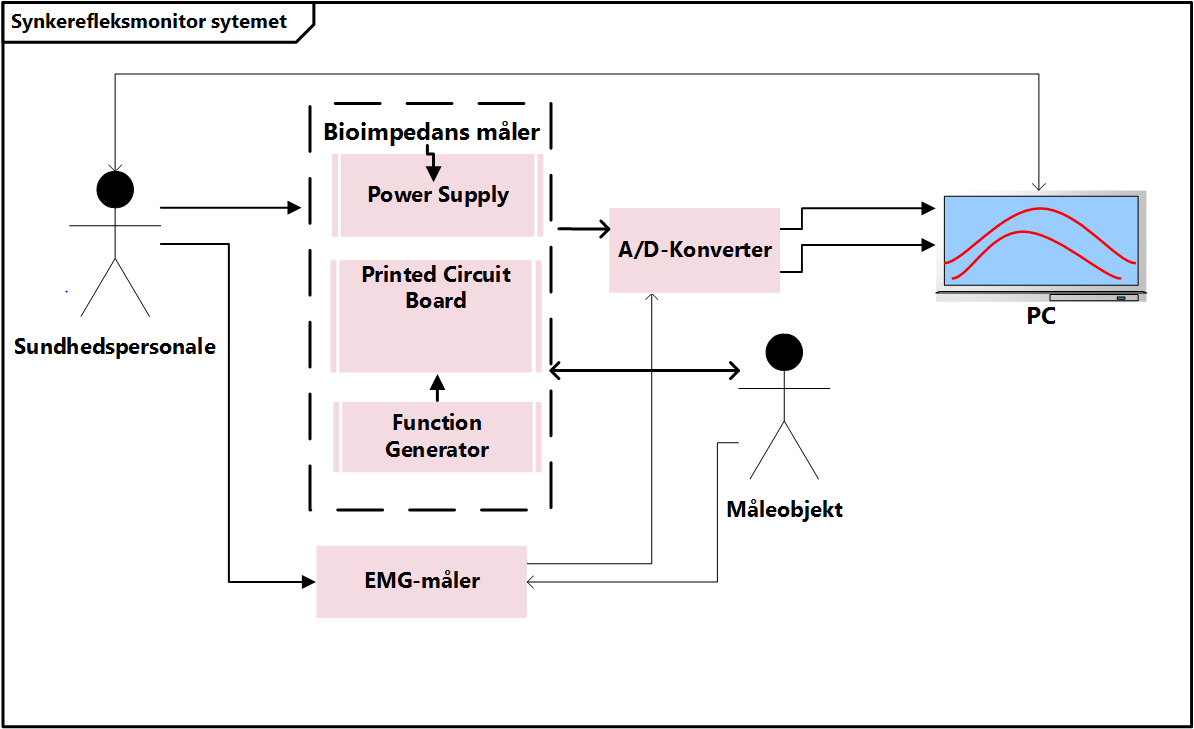
\includegraphics[width=\textwidth]
{Figure/AktoerKontextDiagram}}
\caption{Aktør-kontext diagram}
\label{Use case diagram}
\end{figure}  

\subsection{Aktørbeskrivelse}
\begin{table}[H]
\begin{tabularx}{\textwidth}{l l X}
     Aktørnavn	&	Type		&	Beskrivelse \\ \midrule
     Sundhedspersonale   	&  	Primær  	& 	Sundhedspersonalet tilkobler BI- og EMG-måleren til måleobjektet vha. elektroder, samt starter og afslutter målingen. Yderligere interagerer sundhedspersonalet med en brugergrænseflade.     \\ 			  \addlinespace[2mm]
     Bioimpedans måler	&	Sekundær	& Bioimpedans måleren anvendes til at måle bioimpedans signaler fra måleobjektet  	 \\   \addlinespace[2mm]

  EMG måler	&	Sekundær	&	EMG-måleren anvendes til at måle EMG-signaler fra måleobjektet.
     \\   \addlinespace[2mm]
    
    Måleobjekt	&	Sekundær	&	Måleobjektet er kilden  hvorfra bioimpedans signalerne indhentes. Måleobjektet er tilkoblet til både BI- og EMG-måleren.
     \\   \addlinespace[2mm]
     
 A/D-konverter	&	Sekundær	&	A/D-konverterens funktion er at konvertere analog signaler fra hhv. BI-og EMG-måler  til digital signaler.
     \\   \addlinespace[2mm]      
    PC	&	Sekundær	&	Denne brugergrænseflade bruges til at visualisere de målte signaler i graf form.
     \\   \addlinespace[2mm]
     
   
     \bottomrule                                                                                                                   
    \end{tabularx}
    \caption {Aktørbeskrivelse}
    \label{tab:aktoerbeskrivelse}
	
\end{table}


\section{Funktionelle krav}
\subsection{Use Case diagram}

\begin{figure}[H]
\centering
{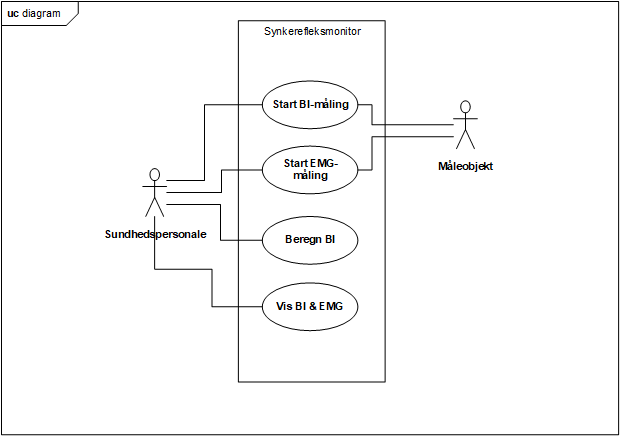
\includegraphics[width=\textwidth]
{Figure/usecasediagram}}
\caption{Use Case diagram}
\label{Use Case diagram}
\end{figure}

Diagrammet i figur \ref{Use case diagram} viser systemets fire Use Cases: Start BI-måling, Start EMG-måling, Beregn BI, Vis BI og EMG. Herunder følger en nærmere
beskrivelse af de enkelte Use Cases, gennem et fully-dressed Use Case skema.




Systemet består af en softwaredel, en A/D-konverter, BI-måler, EMG-måler med tilhørende hardware.
Systemet gør det muligt at foretage en BI- og EMG-måling på et måleobjekt. BI- og EMG-målingerne bliver sendt ind i systemet via A/D-konverter, hvor signalet vises i Matlab. I softwaren er det muligt at få simultane signaler på en graf og samtidig benyttes der algoritme for at vise synkefrekvensen. Denne algoritme undersøger signalet for, ved en omregning fra den kendte spænding og strøm, impedans og dens ændringer som der ligner et synk.
Brugergrænsefladen er det som sundhedspersonalet initierer med, altså hvorfra systemet aktiveres.


\subsection{Use Cases - fully dressed}

\begin{longtabu} to \linewidth{@{}l r X[l]@{}} %UC1%
	{\large \textbf{Use Case 1}} && \\
	\toprule
	Scenarie 				&&	Hovedscenarie\\  
	Navn 					&& 	Start BI-måling\\
	Mål 					&& 	At få foretaget en BI-måling\\
	Initiering 				&& 	Startes af Sundhedspersonale\\
	Aktører 				&& 	Sundhedspersonale (primær), Måleobjekt (sekundær)\\
	Referencer 				&& 	\\
	Samtidige forekomster  	&& 	En BI-måling pr. kørsel \\
	Forudsætninger 			&&	Alle systemer er ledige og operationelle. Elektroder påsat måleobjekt og GUI-vindue er åbent\\ 
	Resultat 				&& 	BI-målingen er blevet foretaget efter ønske\\ \midrule
	Hovedscenarie 			&    1. 	&	Sundhedspersonale trykker på knappen "Start BI-måling"\\				 	
							&    2. 	& 	Systemet foretager målingen indtil der trykkes på knappen "Stop måling" \\[-1ex]
							& 	 3.		&	 Systemet har gemt målingen i en fil \\[-1ex]
                            &&[\textit{Undtagelse 3.a:}] Systemet har ikke gemt målingen\\ \midrule
	Undtagelser 			& 3.a. & Hovedscenarie 1 i Use Case 1 gentages.\\ \bottomrule
                         
	
	\caption{Fully dressed Use Case 1}
	\label{UC1}
\end{longtabu}

\begin{longtabu} to \linewidth{@{}l r X[l]@{}} %UC1%
	{\large \textbf{Use Case 2}} && \\
	\toprule
	Scenarie 				&&	Hovedscenarie\\
	Navn 					&& 	Start EMG-måling\\
	Mål 					&& 	At få foretaget en EMG-måling\\
	Initiering 				&& 	Startes af Sundhedspersonale\\
	Aktører 				&& 	Sundhedspersonale (primær), Måleobjekt (sekundær)\\
	Referencer 				&& 	\\
	Samtidige forekomster  	&& 	En EMG-måling pr. kørsel \\
	Forudsætninger 			&&	Alle systemer er ledige og operationelle. Elektroder påsat måleobjekt og GUI-vindue er åbent\\ 
	Resultat 				&& 	EMG-målingen er blevet foretaget efter ønske\\ \midrule
	Hovedscenarie 			&    1. 	&	Sundhedspersonale trykker på knappen "Start EMG-måling"\\ 				 	
							&    2. 	& 	Systemet foretager målingen indtil der trykkes på knappen "Stop måling" \\[-1ex]
							& 	 3.		&	 Systemet har gemt målingen i en fil \\[-1ex]
                            &&[\textit{Undtagelse 3.a:}] Systemet har ikke gemt målingen\\ \midrule
	Undtagelser 			& 3.a. & Hovedscenarie 1 i Use Case 2 gentages.\\ \bottomrule
	\caption{Fully dressed Use Case 2}
	\label{UC2}
\end{longtabu}

\begin{longtabu} to \linewidth{@{}l r X[l]@{}} %UC1%
	{\large \textbf{Use Case 3}} && \\
	\toprule
	Scenarie 				&&	Hovedscenarie\\
	Navn 					&& 	Beregn BI\\
	Mål 					&& 	At få beregnet BI\\
	Initiering 				&& 	Startes af Sundhedspersonale\\
	Aktører 				&& 	Sundhedspersonale (primær)\\
	Referencer 				&& 	Use Case 1\\
	Samtidige forekomster  	&& 	En BI-beregning pr. kørsel \\
	Forudsætninger 			&&	Use case 1 er foretaget\\ 
	Resultat 				&& 	BI-beregningen er foretaget efter ønske\\ \midrule
	Hovedscenarie 			&    1. 	&	Sundhedspersonale trykker på knappen "Beregn-BI"\\	
							&    2. 	& 	Systemet foretager BI-beregningen\\ 
Undtagelser 			&			& 	-  \\ \bottomrule
	
	\caption{Fully dressed Use Case 3}
	\label{UC3}
\end{longtabu}

\begin{longtabu} to \linewidth{@{}l r X[l]@{}} %UC1%
	{\large \textbf{Use Case 4}} && \\
	\toprule
	Scenarie 				&&	Hovedscenarie\\
	Navn 					&& 	Vis BI \& EMG\\
	Mål 					&& 	At få vist BI- \& EMG-måling over tid på en graf\\
	Initiering 				&& 	Startes af Sundhedspersonale\\
	Aktører 				&& 	Sundhedspersonale (primær)\\
	Referencer 				&& 	\\
	Samtidige forekomster  	&& 	En graf pr. kørsel \\
	Forudsætninger 			&&	Use case 1, 2 og 3 er foretaget\\ 
	Resultat 				&& 	Grafen er vist efter ønske\\ \midrule
	Hovedscenarie 			&    1. 	&	Sundhedspersonale trykker på knappen "Vis BI \& EMG"\\				 	
							&    2. 	& 	Grafen vises i GUI-vinduet\\
	Undtagelser 			&			& 	-  \\ \bottomrule
	
	\caption{Fully dressed Use Case 4}
	\label{UC4}
\end{longtabu}


\section{Ikke-funktionelle krav}

nielsen \cite{NielsenUsabilityUsability}

\subsection{(F)URPS+}

\textbf{Usability}
\begin{enumerate}
\item Sundhedspersonalet skal kunne anvende synkerefleksmonitoren efter 10 minutters instruktion. 
\item Sundhedspersonalet skal kunne efter endt introduktion til synkerefleksmonitoren foretage en måling uden fejl.
\item Sundhedspersonalet skal kunne efter en periode, på en uge væk fra synkerefleksmonitoren, foretage en måling uden fejl.
\item Sundhedspersonalet får mulighed for, at give karakter til GUI-designet på en skala fra 1-5, hvor 5 er yderst tilfredsstillende.
\item Sundhedspersonalet skal kunne aflæse graferne fra GUI'en på 2 meters afstand. 
\end{enumerate}
                                                                                                
\textbf{Reliability}
\begin{enumerate}
\item Det skal maksimalt tage 5 timer at gendanne Synkerefleksmonitor (MTTR - Mean Time To Restore).
\item Synkerefleksmonitor skal have en oppetid uden nedbrud på minimum 1 dag (24 timer) (MTBF - Mean Time Between Failure).  
\item Synkerefleksmonitor skal have en oppetid/køretid på: 
\end{enumerate}


\begin{equation}
Availability = \frac{MTBF}{MTBF+MTTR}\cdot100 = \frac{24}{24+5}\cdot100 = 82,76 \%
\end{equation}

					
\textbf{Performance}
\begin{enumerate}
\item Synkerefleksmonitorens hardware skal kunne tændes indenfor 3 minutter.
\item Synkerefleksmonitorens GUI skal kunne vises indenfor 3 minutter.
\item GUI'ens responstid skal maksimum være 10 sekunder.

\end{enumerate}


\textbf{Supportability}
\begin{enumerate}
\item Sundhedspersonalet skal kunne udskifte batterierne til hardwaren inden for 2 minutter.
\item Sundhedspersonalet skal kunne udskifte elektroderne inden for 2 minutter.
\item Softwaren skal opbygges med lav samhørlighed.
\end{enumerate}

\newpage
\bibliography{Mendeley.bib}
\newpage
\listoffigures
\newpage
\listoftables

\end{document}